% !TEX root = ../eval.tex

\section{Additional results}%
\label{sec:additional_results}



\subsection{Additional TWFE specifications}%
\label{sub:additional_twfe_specifications}

\begin{figure}[H]
    \centering
    \caption{Alternative model specifications}%
    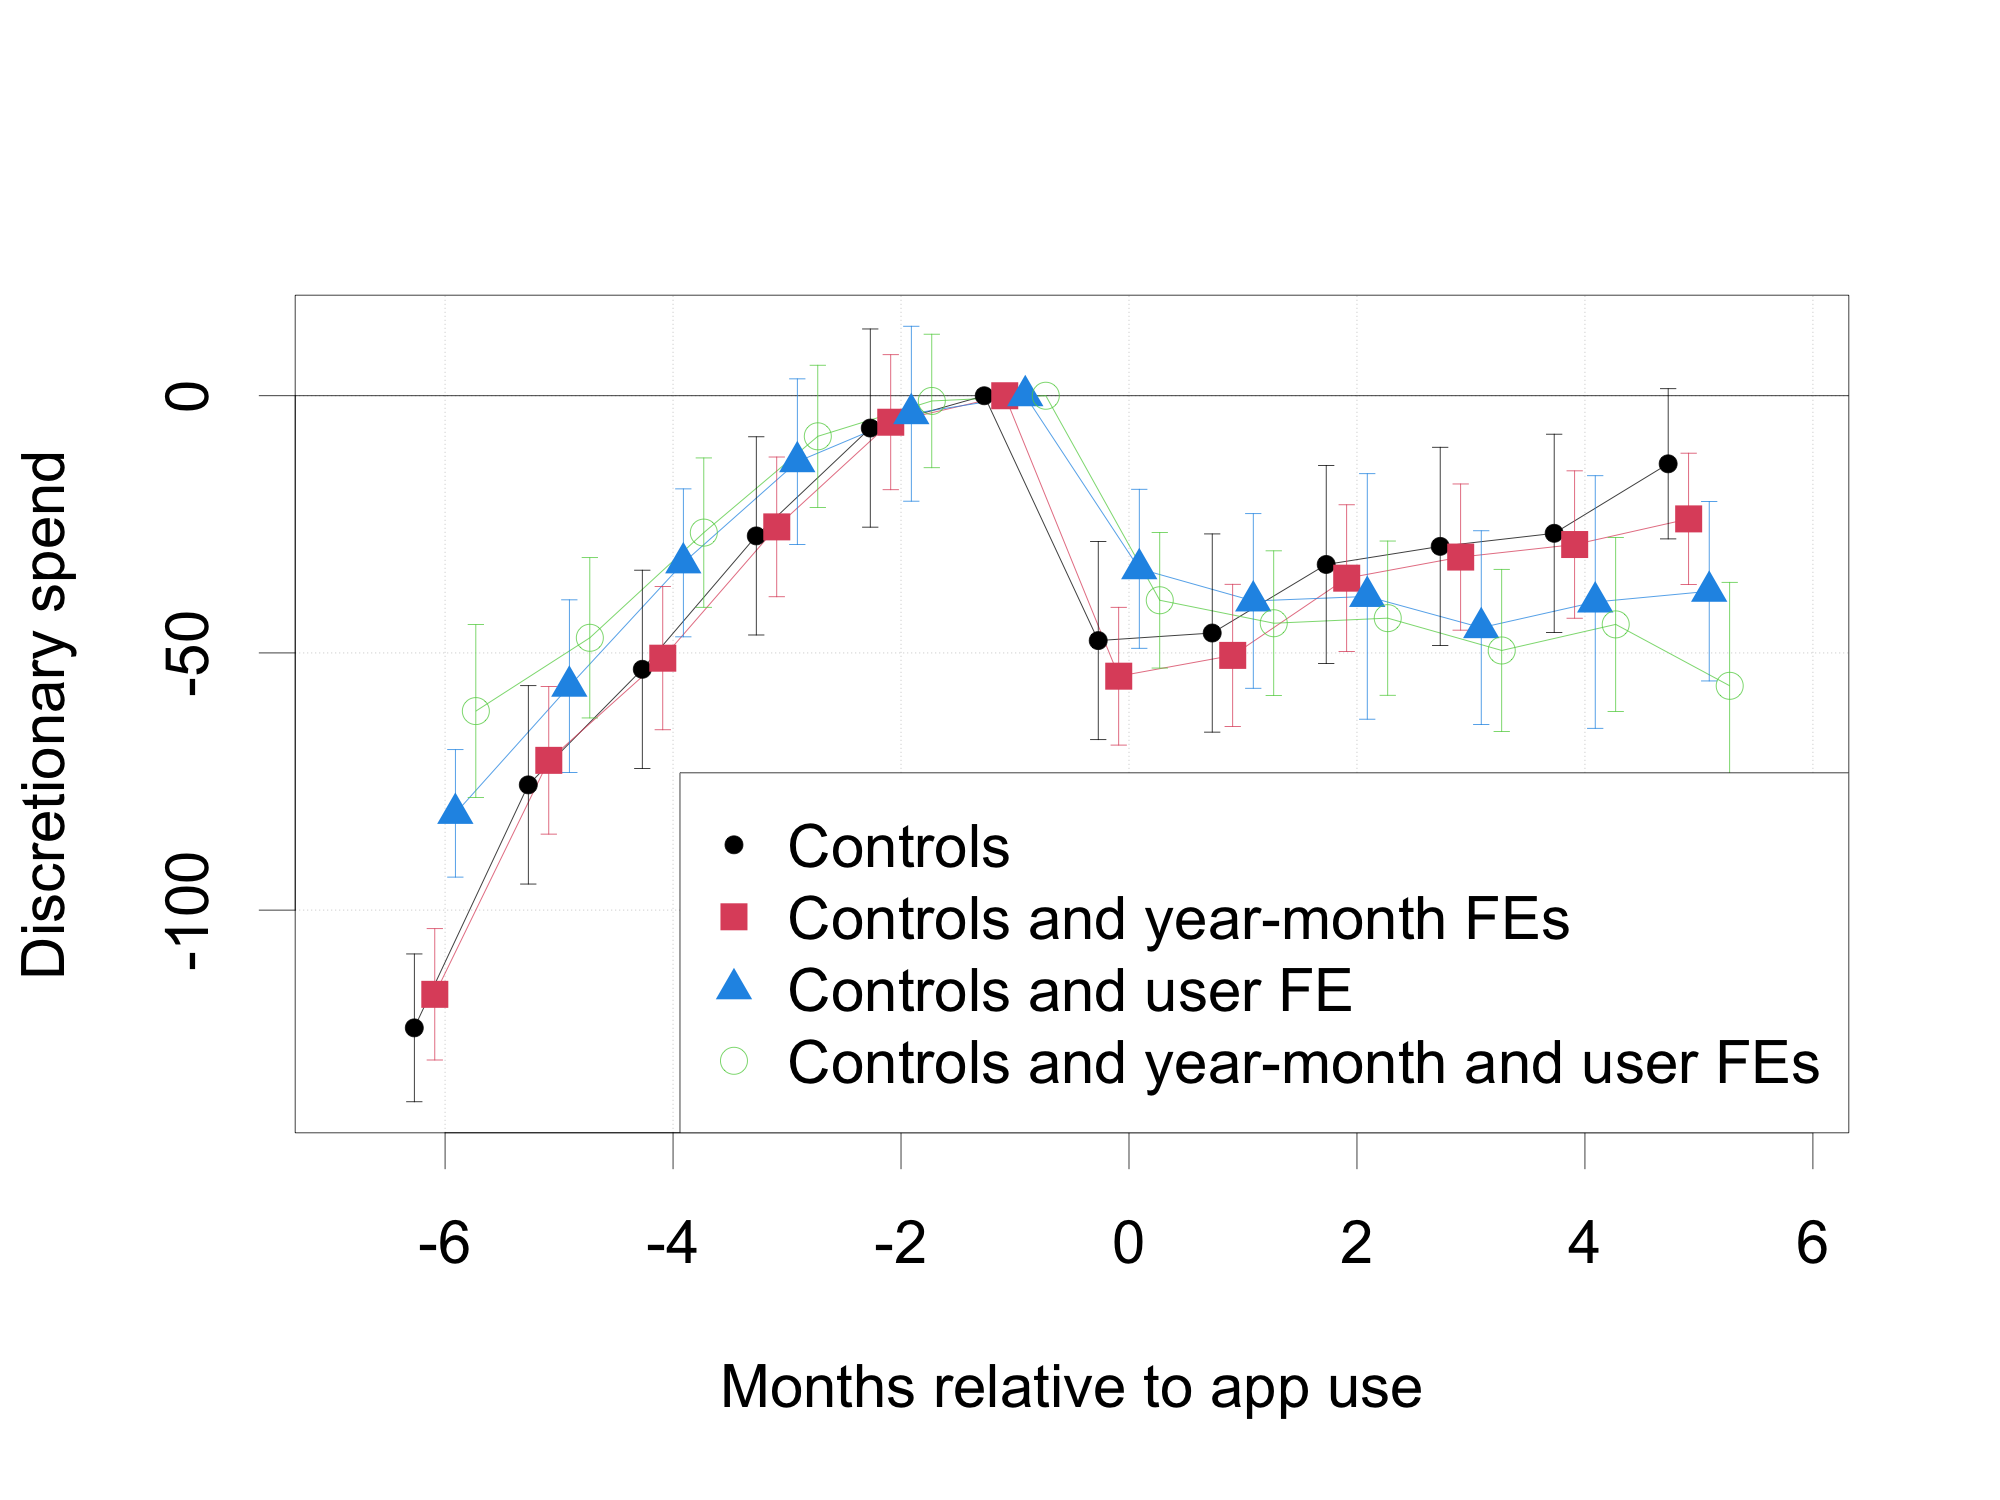
\includegraphics[width=.7\textwidth]{\figdir/dspend_alt.png}
\end{figure}


\begin{table}[htbp]
   \centering
   \tiny
   \begin{threeparttable}[b]
      \caption{\label{tab:dspend_alt} Alternative model specifications}
      \begin{tabular}{lcccc}
         \tabularnewline \midrule \midrule
         Dependent Variable: & \multicolumn{4}{c}{Discretionary spend}\\
         Model:                            & (1)                & (2)                & (3)              & (4)\\  
         \midrule
         \emph{Variables}\\
         Months relative to app use $=$ -6 & -122.89$^{***}$    & -116.38$^{***}$    & -81.19$^{***}$   & -61.31$^{***}$\\   
                                           & [-137.26; -108.52] & [-129.14; -103.61] & [-93.92; -68.47] & [-78.13; -44.48]\\   
         Months relative to app use $=$ -5 & -75.65$^{***}$     & -70.88$^{***}$     & -56.47$^{***}$   & -47.06$^{***}$\\   
                                           & [-94.93; -56.37]   & [-85.23; -56.54]   & [-73.72; -39.23] & [-62.64; -31.47]\\   
         Months relative to app use $=$ -4 & -53.18$^{***}$     & -51.02$^{***}$     & -32.49$^{***}$   & -26.61$^{***}$\\   
                                           & [-72.45; -33.91]   & [-64.94; -37.10]   & [-47.26; -17.72] & [-41.13; -12.09]\\   
         Months relative to app use $=$ -3 & -27.25$^{***}$     & -25.50$^{***}$     & -12.83           & -7.89\\   
                                           & [-46.51; -7.98]    & [-39.08; -11.91]   & [-29.37; 3.72]   & [-21.71; 5.94]\\   
         Months relative to app use $=$ -2 & -6.28              & -5.15              & -3.49            & -1.01\\   
                                           & [-25.55; 12.98]    & [-18.28; 7.98]     & [-20.95; 13.98]  & [-13.00; 11.97]\\   
         Months relative to app use $=$ 0  & -47.60$^{***}$     & -54.52$^{***}$     & -33.64$^{***}$   & -39.76$^{***}$\\   
                                           & [-66.86; -28.34]   & [-67.92; -41.12]   & [-49.51; -17.76] & [-52.94; -26.58]\\   
         Months relative to app use $=$ 1  & -46.13$^{***}$     & -50.48$^{***}$     & -39.90$^{***}$   & -44.23$^{***}$\\   
                                           & [-65.40; -26.86]   & [-64.31; -36.65]   & [-57.33; -22.47] & [-58.30; -30.15]\\   
         Months relative to app use $=$ 2  & -32.80$^{***}$     & -35.47$^{***}$     & -39.02$^{***}$   & -43.24$^{***}$\\   
                                           & [-52.07; -13.53]   & [-49.73; -21.20]   & [-63.52; -14.51] & [-58.23; -28.24]\\   
         Months relative to app use $=$ 3  & -29.28$^{***}$     & -31.36$^{***}$     & -45.09$^{***}$   & -49.52$^{***}$\\   
                                           & [-48.56; -10.01]   & [-45.57; -17.15]   & [-64.44; -25.75] & [-65.30; -33.74]\\   
         Months relative to app use $=$ 4  & -26.75$^{***}$     & -28.93$^{***}$     & -40.10$^{***}$   & -44.45$^{***}$\\   
                                           & [-46.02; -7.47]    & [-43.25; -14.60]   & [-65.31; -14.89] & [-61.37; -27.53]\\   
         Months relative to app use $=$ 5  & -13.23$^{*}$       & -23.94$^{***}$     & -38.01$^{***}$   & -56.39$^{***}$\\   
                                           & [-27.83; 1.37]     & [-36.72; -11.16]   & [-55.92; -20.11] & [-76.52; -36.27]\\   
         Month income                      & 0.02$^{***}$       & 0.01$^{***}$       & 0.02$^{***}$     & 0.01$^{***}$\\   
                                           & [0.02; 0.03]       & [0.01; 0.02]       & [0.02; 0.03]     & [0.00; 0.02]\\   
         Month spend                       & 0.16$^{***}$       & 0.12$^{***}$       & 0.16$^{***}$     & 0.12$^{***}$\\   
                                           & [0.16; 0.16]       & [0.11; 0.12]       & [0.15; 0.17]     & [0.11; 0.12]\\   
         Active accounts                   & 41.94$^{***}$      & 77.85$^{***}$      & 40.80$^{***}$    & 72.39$^{***}$\\   
                                           & [40.39; 43.49]     & [73.30; 82.41]     & [38.37; 43.22]   & [67.89; 76.88]\\   
         Intercept                         & 274.97$^{***}$     &                    &                  &   \\   
                                           & [260.03; 289.91]   &                    &                  &   \\   
         \midrule
         \emph{Fixed-effects}\\
         User ID                           &                    & Yes                &                  & Yes\\  
         Year-month                        &                    &                    & Yes              & Yes\\  
         \midrule
         \emph{Fit statistics}\\
         Observations                      & 188,324            & 188,324            & 188,324          & 188,324\\  
         R$^2$                             & 0.41828            & 0.66337            & 0.42491          & 0.67097\\  
         Within R$^2$                      &                    & 0.28398            & 0.41052          & 0.23935\\  
         \midrule \midrule
         \multicolumn{5}{l}{\emph{Signif. Codes: ***: 0.01, **: 0.05, *: 0.1}}\\
      \end{tabular}
   \end{threeparttable}
\end{table}





\begin{figure}[H]
    \centering
    \caption{Alternative model specifications}%
    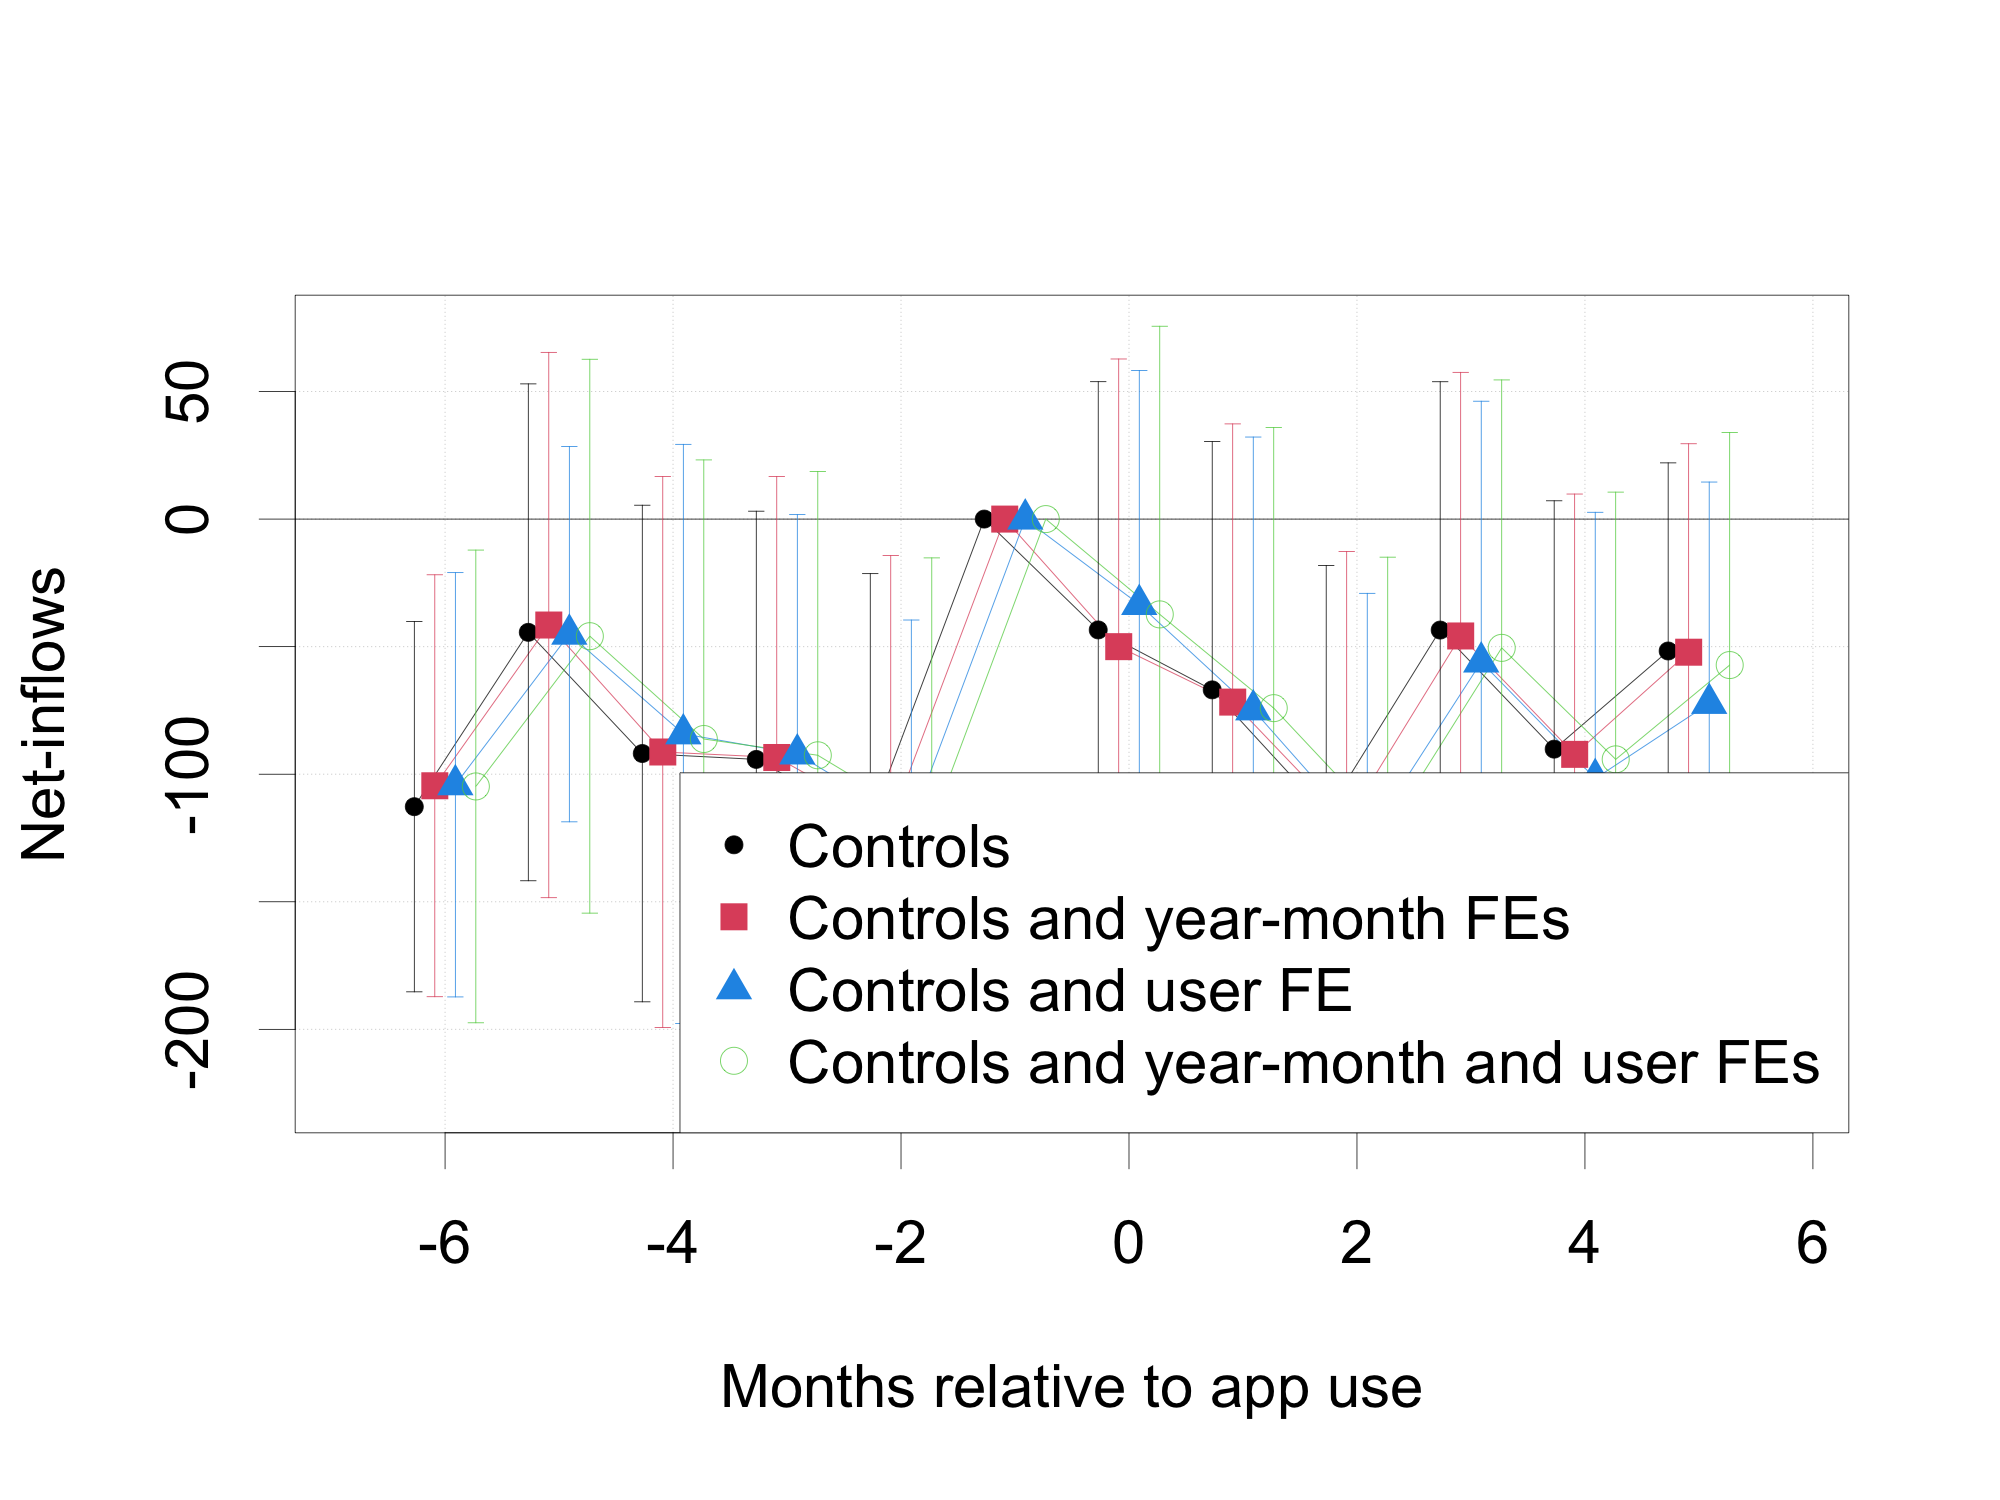
\includegraphics[width=.7\textwidth]{\figdir/netflows_alt.png}
\end{figure}


\begin{table}[htbp]
   \centering
   \tiny
   \begin{threeparttable}[b]
      \caption{\label{tab:netflows_alt} Alternative model specifications}
      \begin{tabular}{lcccc}
         \tabularnewline \midrule \midrule
         Dependent Variable: & \multicolumn{4}{c}{Net-inflows}\\
         Model:                            & (1)               & (2)               & (3)               & (4)\\  
         \midrule
         \emph{Variables}\\
         Months relative to app use $=$ -6 & -112.73$^{***}$   & -104.53$^{**}$    & -104.14$^{**}$    & -104.79$^{**}$\\   
                                           & [-185.30; -40.15] & [-187.23; -21.82] & [-189.54; -18.75] & [-197.45; -12.13]\\   
         Months relative to app use $=$ -5 & -44.39            & -41.53            & -45.12            & -45.90\\   
                                           & [-141.77; 52.99]  & [-148.42; 65.37]  & [-120.66; 30.41]  & [-154.47; 62.67]\\   
         Months relative to app use $=$ -4 & -91.89$^{*}$      & -91.29$^{*}$      & -84.19            & -86.20\\   
                                           & [-189.22; 5.44]   & [-199.28; 16.69]  & [-200.74; 32.37]  & [-195.61; 23.21]\\   
         Months relative to app use $=$ -3 & -94.20$^{*}$      & -93.45$^{*}$      & -92.07$^{*}$      & -92.58\\   
                                           & [-191.50; 3.10]   & [-203.59; 16.70]  & [-188.41; 4.27]   & [-203.84; 18.67]\\   
         Months relative to app use $=$ -2 & -118.68$^{**}$    & -118.36$^{**}$    & -119.19$^{***}$   & -119.53$^{**}$\\   
                                           & [-215.98; -21.39] & [-222.44; -14.29] & [-200.97; -37.41] & [-223.87; -15.19]\\   
         Months relative to app use $=$ 0  & -43.44            & -50.00            & -33.48            & -37.36\\   
                                           & [-140.74; 53.85]  & [-162.78; 62.77]  & [-127.72; 60.75]  & [-150.33; 75.61]\\   
         Months relative to app use $=$ 1  & -66.94            & -71.74            & -74.79            & -74.11\\   
                                           & [-164.24; 30.37]  & [-180.80; 37.33]  & [-184.62; 35.05]  & [-184.14; 35.92]\\   
         Months relative to app use $=$ 2  & -115.51$^{**}$    & -118.47$^{**}$    & -125.25$^{**}$    & -121.66$^{**}$\\   
                                           & [-212.82; -18.19] & [-224.24; -12.70] & [-224.00; -26.50] & [-228.41; -14.90]\\   
         Months relative to app use $=$ 3  & -43.50            & -45.81            & -56.03            & -50.48\\   
                                           & [-140.83; 53.83]  & [-149.17; 57.54]  & [-161.02; 48.97]  & [-155.51; 54.56]\\   
         Months relative to app use $=$ 4  & -90.18$^{*}$      & -92.22$^{*}$      & -101.71$^{*}$     & -94.18$^{*}$\\   
                                           & [-187.52; 7.17]   & [-194.27; 9.84]   & [-208.92; 5.49]   & [-198.96; 10.59]\\   
         Months relative to app use $=$ 5  & -51.70            & -52.18            & -72.25            & -57.21\\   
                                           & [-125.43; 22.03]  & [-133.90; 29.54]  & [-161.36; 16.86]  & [-148.40; 33.97]\\   
         Month income                      & 0.07$^{***}$      & 0.07$^{***}$      & 0.07$^{***}$      & 0.08$^{***}$\\   
                                           & [0.06; 0.08]      & [0.05; 0.10]      & [0.05; 0.09]      & [0.05; 0.10]\\   
         Month spend                       & -0.12$^{***}$     & -0.16$^{***}$     & -0.12$^{***}$     & -0.16$^{***}$\\   
                                           & [-0.13; -0.11]    & [-0.19; -0.14]    & [-0.14; -0.10]    & [-0.19; -0.14]\\   
         Active accounts                   & 38.47$^{***}$     & 72.54$^{***}$     & 37.00$^{***}$     & 72.05$^{***}$\\   
                                           & [30.62; 46.31]    & [56.98; 88.10]    & [24.59; 51.40]    & [56.26; 87.84]\\   
         Intercept                         & 95.97$^{**}$      &                   &                   &   \\   
                                           & [20.52; 171.42]   &                   &                   &   \\   
         \midrule
         \emph{Fixed-effects}\\
         User ID                           &                   & Yes               &                   & Yes\\  
         Year-month                        &                   &                   & Yes               & Yes\\  
         \midrule
         \emph{Fit statistics}\\
         Observations                      & 188,324           & 188,324           & 188,324           & 188,324\\  
         R$^2$                             & 0.00897           & 0.04121           & 0.00948           & 0.04170\\  
         Within R$^2$                      &                   & 0.01022           & 0.00885           & 0.01007\\  
         \midrule \midrule
         \multicolumn{5}{l}{\emph{Signif. Codes: ***: 0.01, **: 0.05, *: 0.1}}\\
      \end{tabular}
   \end{threeparttable}
\end{table}







% \subsection{Static TWFE}%
% \label{sub:static_results}

% \begin{equation}
%     y_{it} = \alpha_i + \lambda_t + \beta D_{it} + \gamma X_{it} + \epsilon_{it}
% \end{equation}

% Notes:
% \begin{itemize}
%     \item Assumption: there are no confounding effects (either time-varying,
%         individual varying, or individual-time varying), so treatment
%         assignment is as good as random.

%     \item With controls, we assume that there are no confounding variables
%         other than the ones we control for.
% \end{itemize}
% 
\begin{table}[htbp]
   \centering
   \tiny
   \begin{threeparttable}[b]
      \caption{\label{tab:reg_static} Static results}
      \begin{tabular}{lcccccccc}
         \tabularnewline \midrule \midrule
         Dependent Variables: & \multicolumn{4}{c}{Net-inflows} & \multicolumn{4}{c}{Discretionary spend}\\
         Model:          & (1)             & (2)             & (3)            & (4)             & (5)              & (6)             & (7)            & (8)\\  
         \midrule
         \emph{Variables}\\
         App use         & 49.96$^{***}$   & 14.21           & 36.60$^{**}$   & 0.22            & 71.37$^{***}$    & 0.84            & 53.08$^{***}$  & -22.61$^{***}$\\   
                         & [19.11; 80.82]  & [-31.50; 59.92] & [6.08; 67.12]  & [-49.16; 49.61] & [65.39; 77.36]   & [-13.45; 15.13] & [43.96; 62.19] & [-33.62; -11.61]\\   
         Month income    & 0.07$^{***}$    & 0.07$^{***}$    & 0.08$^{***}$   & 0.08$^{***}$    & 0.02$^{***}$     & 0.02$^{***}$    & 0.01$^{***}$   & 0.01$^{***}$\\   
                         & [0.06; 0.08]    & [0.05; 0.09]    & [0.05; 0.10]   & [0.05; 0.11]    & [0.02; 0.02]     & [0.02; 0.03]    & [0.00; 0.02]   & [0.00; 0.01]\\   
         Month spend     & -0.12$^{***}$   & -0.12$^{***}$   & -0.16$^{***}$  & -0.16$^{***}$   & 0.16$^{***}$     & 0.16$^{***}$    & 0.12$^{***}$   & 0.12$^{***}$\\   
                         & [-0.13; -0.11]  & [-0.14; -0.10]  & [-0.18; -0.14] & [-0.19; -0.13]  & [0.16; 0.16]     & [0.15; 0.17]    & [0.11; 0.12]   & [0.11; 0.12]\\   
         Active accounts & 38.80$^{***}$   & 37.49$^{***}$   & 70.26$^{***}$  & 68.78$^{***}$   & 46.84$^{***}$    & 42.56$^{***}$   & 86.86$^{***}$  & 75.18$^{***}$\\   
                         & [30.04; 47.56]  & [23.46; 51.53]  & [53.08; 87.44] & [46.71; 90.85]  & [45.14; 48.54]   & [39.57; 45.55]  & [81.78; 91.95] & [70.63; 79.72]\\   
         Intercept       & -6.05           &                 &                &                 & 171.35$^{***}$   &                 &                &   \\   
                         & [-41.06; 28.95] &                 &                &                 & [164.56; 178.14] &                 &                &   \\   
         \midrule
         \emph{Fixed-effects}\\
         Year-month      &                 & Yes             &                & Yes             &                  & Yes             &                & Yes\\  
         User ID         &                 &                 & Yes            & Yes             &                  &                 & Yes            & Yes\\  
         \midrule
         \emph{Fit statistics}\\
         Observations    & 148,932         & 148,932         & 148,932        & 148,932         & 148,932          & 148,932         & 148,932        & 148,932\\  
         R$^2$           & 0.00879         & 0.00932         & 0.03981        & 0.04033         & 0.41708          & 0.42534         & 0.66066        & 0.66973\\  
         Within R$^2$    &                 & 0.00869         & 0.00933        & 0.00922         &                  & 0.41021         & 0.28163        & 0.23660\\  
         \midrule \midrule
         \multicolumn{9}{l}{\emph{Signif. Codes: ***: 0.01, **: 0.05, *: 0.1}}\\
      \end{tabular}
   \end{threeparttable}
\end{table}





